\documentclass[9pt,twocolumn,twoside,lineno]{article}
%\templatetype{pnasresearcharticle}

%\usepackage[margin=.8in]{geometry}
%\usepackage{graphicx}
%\usepackage{amsmath}
%\usepackage{amssymb}
%\usepackage{titlesec}
%\usepackage[numbers]{natbib}
%\usepackage{sidecap, caption}
\usepackage{subcaption}
\usepackage[figuresleft]{rotating}
\usepackage{fixme}

\usepackage{tikz}
\usetikzlibrary{arrows,calc,matrix, arrows.meta,automata}
\tikzset{
%Define standard arrow tip
>=stealth',
%Define style for different line styles
help lines/.style={dashed, thick},
axis/.style={<->},
important line/.style={thick},
connection/.style={thick, dotted},
}

\newcommand{\at}{\makeatletter @\makeatother}
%\titlespacing*{\section}
%{0pt}{2ex}{0ex}
%\titlespacing*{\subsection}
%{0pt}{2ex}{0ex}
%\titlespacing*{\subsubsection}
%{0pt}{2ex}{0ex}
%\font\myfont=cmr12 at 16pt

\graphicspath{{../plots/}}

\title{The Wisdom and Persuadability of Threads}

% Use letters for affiliations, numbers to show equal authorship (if applicable) and to indicate the corresponding author
%\author{Robin Engelhardt}
%\author{Jacob Stærk-Østergaard}
%\author{Vincent F. Hendricks}

%\begin{affiliations}
% \item Center for Information and Bubble Studies, Department of Communication, University of Copenhagen, Karen Blixens Plads 8, DK-2300 Copenhagen S.
%\end{affiliations}


% Please give the surname of the lead author for the running footer
%\leadauthor{Engelhardt} 

% Please add here a significance statement to explain the relevance of your work
%\significancestatement{Online discussion threads are important means for individual decision-making as well as for aggregating collective judgments. Empirical and theoretical investigations of this `wisdom of crowds' are currently ambivalent about the role played by social information. While some findings suggest that social information undermines crowd accuracy due to correlated judgment errors, others show that accuracy improves. We demonstrate that, for difficult tasks, seeing preceding estimates aids individual decision-making as well as collective accuracy in pristine threads, but not in manipulated threads where participants only see the most extreme estimates. By assigning a persuadability score to each estimate, we additionally show that persuadability depends on task difficulty as well as on the amount of social information received.
%}

% Please include corresponding author, author contribution and author declaration information
%\authorcontributions{R. E. designed the experiment and analyzed the data and contributed as lead author, J. S-Ø. analyzed the data and contributed as co-author, V.F.H. contributed as the co-author and as the project manager.}
%\authordeclaration{The authors declare no conflict of interest.}
%%\correspondingauthor{\textsuperscript{1}ORCID: 0000-0002-7162-0990}
%\correspondingauthor{\textsuperscript{1}To whom correspondence should be addressed. E-mail: robin\at hum.ku.dk}


% Keywords are not mandatory, but authors are strongly encouraged to provide them. If provided, please include two to five keywords, separated by the pipe symbol, e.g:
%\keywords{collective intelligence $|$ magnitude estimation $|$ decision-making $|$ discussion threads $|$  social networks} 

%\maketitle
\renewcommand{\maketitlehookd}{%
\begin{abstract}
\noindent 
Social decision-making is increasingly relying on digitized aggregates of people’s opinions and judgments. These aggregates are frequently maintained as threads, i.e. as sequences of posts on a website. While it has been shown that knowledge of thread aggregates can distort individual decision-making, it is unknown how seeing preceding posts in a thread may influence collective accuracy, i.e. the wisdom of threads, as well as individual persuadability. We investigate experimentally the accuracy of threads in which people make magnitude estimations of varying difficulty and varying degrees of social information in the form of visible previous estimates. We find a significant increase in collective accuracy for high difficulties and high levels social information in pristine threads, while collective accuracy declines quickly under the same conditions in manipulated threads. Using gaussian mixture models we assign a persuadability score to each participant, and show that persuadability generally increases with task difficulty and with the amount of social information. In the case of strong manipulation, we may see a split between a minority of persuadables and a majority of skeptics.
\end{abstract}
}

%\begin{abstract}
%Social decision-making is increasingly relying on digitized aggregates of people’s opinions and judgments. These aggregates are frequently maintained as threads, i.e. as sequences of posts on a website. While it has been shown that knowledge of thread aggregates can distort individual decision-making, it is unknown how seeing preceding posts in a thread may influence collective accuracy, i.e. the wisdom of threads, as well as individual persuadability. We investigate experimentally the accuracy of threads in which people make magnitude estimations of varying difficulty and varying degrees of social information in the form of visible previous estimates. We find a significant increase in collective accuracy for high difficulties and high levels social information in pristine threads, while collective accuracy declines quickly under the same conditions in manipulated threads. Using gaussian mixture models we assign a persuadability score to each participant, and show that persuadability generally increases with task difficulty and with the amount of social information. In the case of strong manipulation, we may see a split between a minority of persuadables and a majority of skeptics.
%\end{abstract}

\dates{This manuscript was compiled on \today}
%\doi{\url{www.pnas.org/cgi/doi/10.1073/pnas.XXXXXXXXXX}}

\begin{document}

\maketitle
\thispagestyle{firststyle}
\ifthenelse{\boolean{shortarticle}}{\ifthenelse{\boolean{singlecolumn}}{\abscontentformatted}{\abscontent}}{}

\dropcap{S}ocial information in the form of opinions and judgments by other people is sampled sequentially. We read the news, hear rumors, listen to debates on TV, and flip through comments on social media platforms and blogs. These activities inform us and influence our decisions, but researchers still debate the conditions under which these types of social information help us make better decisions \cite{woolley2010evidence, gurccay2015power, becker2017network, jayles2017social}, lead us astray \cite{caplan2011myth, lorenz2011social, minson2012cost, king2011true, le2018endogenous}, or just make us confused at a higher level \cite{salganik2006experimental, salganik2009web}.

Collective estimates of a diverse group of people can outperform the majority of its members because any random confusion at the individual level is likely to average out and let the most accurate estimate prevail \cite{galton1907vox, muth1961rational, surowiecki2005wisdom, hong2008some}. Then again, confusion is not always randomly scattered around the truth. Systematic biases in individual perception may create measurable disruptions in the wisdom of crowds \cite{izard2008calibrating, nash2014curious, kao2018counteracting}. Social information can add to those biases and create cascades, echo chambers, bandwagoning and herd behavior \cite{anderson1997information, bikhchandani1992theory, bakshy2015exposure, banerjee1992simple}. Partially sampled social information may lead to rich-get-richer dynamics \cite{barabasi1999emergence} and to belief misattributions, which uphold harmful social practices despite being rejected by a majority of people \cite{katz1931students, darley1968bystander, ross1977false, noelle1974spiral, lee2019homophily}. Social information may also have been intentionally filtered or manipulated in various ways, for instance through group pressure \cite{asch1951effects}, algorithmic filtering \cite{pariser2011filter}, false cues \cite{salganik2006experimental, muchnik2013social, hanson1996hits}, or simply by plain misinformation \cite{hendricks2018reality}, often with highly detrimental consequences for our economy and our health.

Observational data of decision-making processes is acutely sensitive to the social context in which people find themselves. Thus, researchers find it difficult to separate observational data into its social and individual components. How may we know how much weight an individual puts on her own ‘independent’ estimate relative to the weight put on the estimates by others? Randomized experimental studies have attempted to solve this problem by first letting participants make a magnitude estimate of an object without social information (\textit{ex ante}), and subsequently ask them to revise their estimate after having received information about other people’s estimates of that object (\textit{ex post}) \cite{becker2017network, jayles2017social, lorenz2011social, sniezek1995cueing, mavrodiev2013quantifying}. This double elicitation paradigm presumes that people change their mind because of the social information they have received. Other studies, however, have shown that people routinely can change their mind all by themselves, and that it may be more correct to assume an `inner crowd' in the sense that people sample randomly from a probability distribution in their own mind \cite{vul2008measuring, herzog2009wisdom, herzog2014harnessing}. Such a psychological mechanism - and maybe others such as hedging strategies due to anticipated regrets \cite{bell1982regret}, and/or disappointments \cite{loomes1986disappointment} - make it difficult to differentiate between `inner' samples and `outer' influences, and it may therefore be desirable to develop an alternative framework that is able infer the extend of individual bias and social influence from a single estimation task.

We propose to use probabilistic gaussian mixture models (GMMs) since they have properties that are highly valuable in the context of crowd aggregation research. First, GMMs are comprised of several Gaussians which fit well to the right-skewed, multimodal, and long-tailed distributions emerging from free response elicitations. Second, GMMs associate a measure to each data point, describing the influence of social information on that particular participant. This measure aids us in associating participants with sub-populations in the data related to how people act under available social information, without using any prior knowledge of these sub-populations. Finally, as a statistical model, GMMs provide confidence bounds to the estimates, which further adds a measure of model certainty.

We also propose the experimental mechanism of dot-guessing games \cite{horton2010dot}, where participants guess the number of dots in an image. While dot estimations have been used previously in numerosity experiments \cite{minturn1951effect, indow1977scaling, krueger1982single} they have only recently been proposed as useful ‘model organisms’ for crowd aggregation research \cite{horton2010dot, ugander2015wisdom} due to their advantages in terms of cultural neutrality, resistance to expertise and/or prior knowledge, and their qualities as captchas \cite{von2008recaptcha}. In addition, dot estimation tasks are easy to implement and easy to understand. Most importantly, they have an objective solution and are tunable, allowing for nearly-continuous difficulty levels and performance measures.

\section*{Experimental Design}
We collected a total of 11,748 estimates from 6,196 unique participants on Amazon Mechanical Turk. 5,990 estimates were collected from participants placed in 12 different threads where they successively estimated the number of dots, $d \in \{55,148,403,1097\}$, in an image, while seeing $v \in \{1,3,9\}$ \textit{preceding} estimates (historical threads). Another 3,934 estimates were collected from participants who were placed in 12 other threads and shown the same images while seeing the $v \in \{1,3,9\}$ \textit{highest} estimates made so far (manipulated threads). Finally, 1.824 estimates were collected from participants who were shown the same images, but with $v=0$, corresponding to control conditions for each $d$ containing no social information. 

We interpret the number of dots, $d$, as the \textit{task difficulty}, while the number of visible previous estimates, $v$, is interpreted as the \textit{degree of social information}. Participants were placed randomly in one of the 28 threads ($2 \times 3 \times 4$ + 4 controls)  and made their estimate one after another. In order to keep the estimates in a somewhat realistic range, participants could not submit numbers below 10 and above 1.000.000. No participant who had seen a certain image would be able to participate in another thread containing the same image again. In addition to a participation fee and a variable waiting fee, all participants in all threads received a bonus of \$1 if their estimate was within 10\% of the true value. See the Materials and Methods section and the Appendix for additional information about the experimental design.

\section*{Methods}
Free response elecitation of absolute values is known to create right-skewed distributions with long tails, which inflate the means. While it is still debated which measure is best suited to aggregate such data \cite{kao2018counteracting}, we follow the lead of Galton \cite{galton1907vox} and focus on the median as it is easy to interpret, robust against outliers, and best expresses the opinion of the crowd in the sense that the majority deems every other estimate as too high or too low. For the statistical analysis of thread aggregates, we therefore compare the log-ratio of thread medians, $y_{dv}=\log(M_{(d,v)}/d)$, using a linear normal model to quantify differences between threads in terms of $\log(d)$ and $v$, the latter as a categorical variable (see Materials and Methods). 

\begin{figure}[h]
\centering
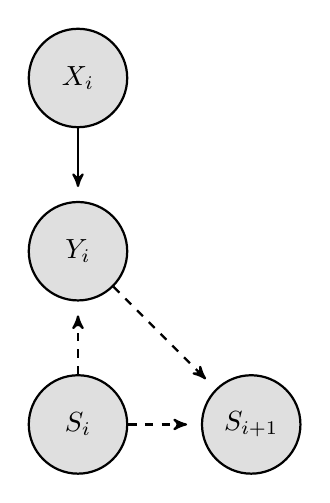
\begin{tikzpicture}[->,>=stealth',shorten >=5pt,auto,node distance=2.2cm, thick,main  
node/.style={circle,fill=gray!25,draw,font=\sffamily\bfseries, minimum size=1.25cm}]
	\node[main node] (x1) {$X_{i}$};
	%\node[main node] (x2) [right of=x1] {$X_{i+1}$};
	\node[main node] (y1) [below of=x1] {$Y_{i}$};
	%\node[main node] (y2) [below of=x2] {$Y_{i+1}$};
	\node[main node] (m1) [below of=y1] {$S_{i}$};
	\node[main node] (m2) [right of=m1] {$S_{i+1}$};
	\path[every node/.style={font=\sffamily\small}]
    		%(m1) edge [dashed, bend right=30] (m2) 
    		(m1) edge [dashed] (m2) edge [dashed] (y1)
		%(m2) edge [dashed] (y2)
		(y1) edge [dashed] (m2) 
		(x1) edge (y1)
		%(x2) edge (y2)
  		;
	\end{tikzpicture}
	\caption{Gaussian Mixture Model dependencies with the observed estimate $Y_i$ by participant $i$, the latent state variable $X_i$, and the social information $S_i$ when consisting of preceding estimates. Dashed lines are connections that depend on the number of views $v$. When $v=0$, $S_i$ is omitted from the model, when $v=1$ then $S_i\to Y_i$ and $Y_i\to S_{i+1}$. For $v>1$ then $S_i\to S_{i+1}$ is added.}
\label{fig:model}
\end{figure}

The effects of social information on individual descision-making are analysed using probabilistic gaussian mixture models on the log-ratio of individual estimates $Y_i$ with the geometric mean of the social information as the explanatory variable $S_i$. Model dependecies are shown in Figure~\ref{fig:model}. 

The model assigns to each participant a \textit{persuadability score}, $\beta^w$, which is high when people are highly influenced by the social information they can see, and small when people are not influenced, or when they are skeptical about the information (see Materials and Methods and SI text for details). 

\begin{figure*}[t]
\centering
	\begin{subfigure}[t]{.46\linewidth}
		\centering
		\includegraphics[width=1\linewidth]{med_confidence_h.pdf}	
		\caption{\footnotesize Historical threads.}
		\label{fig: median confidence bounds - historic}
	\end{subfigure}
	\begin{subfigure}[t]{.46\linewidth}
		\centering
		\includegraphics[width=1\linewidth]{med_confidence_m.pdf}		
		\caption{\footnotesize Manipulated threads.}
		\label{fig: median confidence bounds - manipulated}
	\end{subfigure}
	\caption{\textbf{Thread accuracy}. Relationship between median log-ratio $y_{dv}$ and $\log(d)$ with 95\% confidence bounds (shaded areas). Colors represent the number of visible estimates, $v$. There is a clear relation between $d$ and $v$ in both thread types showing that social information plays a dual role in difficult tasks: When $v$ is large, unmanipulated social information \textbf{(a)} counteracts underestimation bias and improves thread accuracy. When the social information is manipulated \textbf{(b)}, however, a strong overestimation bias emerges for large $v$. The red lines corresponding to the control groups with $v=0$ are identical in both plots.}
	\label{fig: median confidence bounds}
\end{figure*}


\section*{Results}
In accordance with previous findings, participants do well in tasks without social information, especially when estimating small numbers. For higher difficulties estimates vary widely and biases become substantial \cite{indow1977scaling, izard2008calibrating, krueger1982single, krueger1984perceived, kao2018counteracting}. The median tends to underestimate the true value and the mean tends to overestimate the true value. Summary statistics of all 28 treatments can be inspected graphically and in table format in the supplementary information (SI).

\subsection*{Analysis of thread performance}
The relationship between the observed median log-ratio $y_{dv}$ and the number of dots $d$ were found to be optimal, according to quantile-quantile plots (see SI-text), when modeling $y_{dv}$ against $\log{d}$. We thus quantify the overall differences between threads in terms of the log-ratio of their medians, $y_{dv}=\log(M_{(d,v)}/d)$, as a function of $\log(d)$ and $v$. Historical and manipulated threads are modelled separately.

Figure \ref{fig: median confidence bounds - historic} shows that the collective performance of historical threads declines significantly with increasing task difficulty, but improves when the social information is substantial. In contrast to \cite{lorenz2011social, king2011true, minson2012cost} and in concert with \cite{gurccay2015power, becker2017network, jayles2017social, farrell2011social} these findings support the claim that crowds indeed may become wise under (pristine) social influence. It should be noted, however, that the overlapping confidence intervals reveal where thread performances are comparable. Thus, the negative effects of task difficulty and the positive effects of social information are only discernible in situations where people have hard problems to solve and at the same time have plenty of social information available. In fact, the median estimate of historical threads with $v=9$ is `wise' in the sense of being statistically indistinguishable from the true value for all task difficulties $d$.

In manipulated threads, Fig.\ref{fig: median confidence bounds - manipulated}, the manipulation gives a large positive bias for $v=3,9$ which increases with $d$, implying that when a task becomes more demanding, the amount of (filtered) social information has a highly detrimental impact on thread performance. For $v=1$ there is still a small negative trend, meaning that the manipulation is not very effective. This resonates well with findings in \cite{jayles2017social}, who show that providing a moderate amount of incorrect information can counterbalance underestimation bias and improve collective performance. 

\subsection*{Analysis of Persuadability} 
A GMM was fitted to all threads after removing estimates below the 2.5\% and above the 97.5\% quantiles. For each model, standardized residuals are evaluated visually using quantile-quantile plots against a standard normal $\mathcal{N}(0,1)$, see SI-text. These plots reveal that models using $k=2,3,4$ states fit the data quite well, with only a few models displaying a less adequate fit.

\begin{figure*}[!h]
	\centering
	\begin{subfigure}{.44\linewidth}
		\centering
		\includegraphics[width=1\linewidth]{C:/Users/hjl161/Documents/Conferences/2020/ci2020/abstract/ci-2018-latex/images/h10971.pdf}
		%\includegraphics[width=1\linewidth]{/thread_history_1097_1.pdf}
		%\includegraphics[width=.48\linewidth]{info_history_1097_1.pdf}
		\caption{\footnotesize History thread with $d=1097$ and $v=1$}
		\label{fig: h=history d=1097, v=1}
	\end{subfigure}
	\begin{subfigure}{.44\linewidth}
		\centering
		\includegraphics[width=1\linewidth]{C:/Users/hjl161/Documents/Conferences/2020/ci2020/abstract/ci-2018-latex/images/m10979.pdf}
		%\includegraphics[width=1\linewidth]{thread_max_1097_9.pdf}
		%\includegraphics[width=.48\linewidth]{info_max_1097_9.pdf}
		%\includegraphics[width=.48\linewidth]{beta_max_1097_9.pdf}
		\caption{\footnotesize Manipulated thread with $d=1097$ and $v=9$}
		\label{fig: h=max d=1097, v=9}
	\end{subfigure}
	\begin{subfigure}{.1\linewidth}
		\centering
		\includegraphics[width=1\linewidth]{betascale_vertical.pdf}
	\end{subfigure}
	\caption{The left hand side shows three plots of a historical thread with $d=1097$ and $v=1$, and the right hand side shows three plots of a manipulated thread with $d=1097$ and $v=9$. Top plots shows the log-ratio estimates over time (observation no.), with the geometric mean of the social information shown by a dotted line. Bottom left plots show the log-ratio of the estimates as a function of the log-ratio of the social information, indicating how differently participants use their social information. Bottom right plots show the cumulative distribution of individual $\beta^w$'s with 95\% intervals derived from the fitted models and added interquartile values of $\beta^w$.}
\label{fig: social influence}
\end{figure*}

In Fig. \ref{fig: social influence} two exemplary threads show how our model framework can reveal interesting features of the data (more threads are analyzed in the SI). Each thread is presented by three figures. The top figures shows the log-ratio of estimates as the thread evolves over time, with the geometric mean of the social information shown by a dotted line. Each estimate has an associated color, given by the persuadability score $\beta^w$, which measures the effect of the social information on each participant. A high value ($\beta^w>0.6$) in blue colors implies a large social influence effect, a low value ($\beta^w\approx 0$) in red implies little or no effect, and a medium value ($\beta^w \approx 0.4$) in brown and green colors suggests a compromise between the two extremes. The RGB color scale (right) is the same among all threads and plots. The bottom left plots shows the log-ratio of the estimates as a function of the log-ratio of the social information, indicating how differently people use their social information: The more they align with the identity line, the more they tend to follow the social information. 

The bottom right plots show the cumulative distribution of the persuadability scores with 95\% confidence intervals derived from the fitted model. They clearly show how people can be categorized into those ‘sleeping dogs’ or ‘lost causes’ \cite{devriendt2018literature} in red that do not take other peoples estimates into account, the `persuadables' that tend to follow others, and a large group of green `compromisers', who try to strike a balance between what they see others have guesses, and what they believe themselves. Of course, such labels are only proximate. Given a participant has a personal estimate much in line with the social information seen, this participant may be labelled as a persuadable or as a compromiser, when in fact this is only partially true. In general, however, the distributions are remarkable stable across threads, which suggests that people indeed may be partitioned into such overlapping response types.



\subsubsection*{A Closer Look at Manipulated Threads}
What becomes abundantly clear when examining the results from the GMMs, is a sharp contrast between how people act in pristine historical threads where they can see the \textit{preceding} estimates, and how people act in manipulated threads, where they see only a \textit{filtered selection} of previous estimates, in our case the highest ones made so far. When task difficulty is low and $v=1$, participants are not much influenced, no matter whether they see the preceding or highest estimate in their thread. But as soon as visibility increases, more people tend to follow – or at least compromise (see supplementary data analysis in the SI-text). This indicates that there is a weak bandwagon effect at work \cite{bikhchandani1992theory, nadeau1993new, lee2018understanding}, making it more likely for people to follow others the more people have done so already. 

If $d$ is increased as well, the number of persuadables increases. This general pattern of correlations between high (d,v) and high persuadability continues, and in the thread with the highest difficulty and highest visibility, Figure~\ref{fig: h=max d=1097, v=9}, we see huge errors in most estimates. In the beginning, the manipulation may not as pronounced, and participants go along for quite a while. However, as the thread evolves, the red group of skeptics increases, and a prototypical polarization emerges between enthusiastic persuadables and the rest of the thread population, which is visible in the transistional `kink' in the $\beta^w$-distribution around the 65\% quantile in the bottom right plot of Figure~\ref{fig: h=max d=1097, v=9}. It shows that at least 30\% of the participants in this thread are strongly influenced by the filtered information given to them.

%\textcolor{red}{
%Here it would be nice to show an aggregated result across threads from our GMM framework. Could we for instance show in a graph of the $\tilde{\beta}$ interquartiles (25\%, 50\%, 75\%) as a function of $d$ and $v$ for manupulated/unmanipulated threads?
%}

\section*{Conclusion}
We have tried to shed light on the question of whether social information can improve crowd wisdom or whether it can not. Our answer is both. Social information in online estimation threads does help when people have difficult questions to answer and when the information available to them is pristine and representative. However, if the social information is filtered and not representative of the thread population, it becomes manipulative and may fool a substantial proportion of people, which, of course, interferes with any aspiration to harness the powers of collective intelligence. 

Moving from the aggregate to the individual level, we find that people can be assigned a persuadability score by using Gaussian mixture models. Persuadability generally increases with task difficulty and with the amount of social information provided to them. In the case of strong manipulations, we may see a split between a minority of persuadables and a majority of skeptics.

We do not know how much these influencing effects are transferable to other domains. However, due to the general nature of dot estimations, we suspect the effects to be substantial in other settings as well, and also for other questions – especially for those that are more emotional, subjective and political in nature. In computational social science and decision-making research,  there is an acute need to further investigate the types of ‘disturbances’ in online threads and crowds, such as filters, rankings, likes, and recommendations, as well as the types of reaction to those disturbances. To the end of designing future collective intelligence systems, we need to be vigilant about the way social information is gathered and framed. Crowd knowledge and thread wisdom is very fragile, and can only be maintained and nurtured with strong controls upon the way it is cultivated and recovered.

\matmethods{\subsection*{Experimental design and data collection} All experiments were coded in otree 2.1 \cite{chen2016otree}. The code itself is designed along the same lines as the classical information cascade experiments by Anderson and Holt \cite{anderson1997information}. A participant makes an estimate, and the next one receives the information about the estimate of the previous participant(s). Thus, the main technical issue is that only one person at a time can make a decision while others wait. As soon as a participant finishes and leaves the choice page, the next participant enters while all subsequent participants still have to wait. We obtained a total of 11.748 estimates from 6.169 unique participants. Any dot-image was only seen once by a participant, i.e. we had a total of 3.157 participants seeing only one image, 1.259 participants seeing two images, 1.047 participants seeing three images, and 733 participants seeing all four images (either in the unmanipulated or manipulated conditions and with $v \in \{0, 1, 3, 9\}$). After providing informed consent, participants waited in a ‘waiting room’ until the ‘choice room’ became available. When entering the choice room participants could see an image $d$ together with $v \in \{0,1,3,9\}$ previous estimates. After making an estimate, participants were thanked and paid a participation fee of \$0.10 and bonus of \$1 if their estimate was within 10\% of the true number. The average time used was less than two minutes, see SI Appendix for screenshots and detailed descriptions of the experimental design and setup.

\subsection*{Analysis of thread medians}
For observed medians $M_{dv}, d\in \{55,148,403,1097\}, v \in \{0,1,3,9\}$ the log ratios $y_{dv} = \log (M_{dv}/d)$ were modeled using a linear normal model. For a given thread, $\log{d}$ was used as a quantitative variable whereas $v$ was used as a categorical factor. Hence, $y_{dv} = \alpha_v+\beta_v\log{d}+\varepsilon_{dv}$, $\varepsilon_{dv} \sim \mathcal{N}(0,\sigma^2)$. Models were fitted separately to historical and manipulated threads to allow for different variance estimates $\hat{\sigma}^2$ between these groups. Goodness of fit was assessed by quantile-quantile (QQ) plots of the residuals (see appendix ref??).

\subsection*{Analysis of social influence}
The influence of social information was analyzed using a Gaussian Mixture Model (GMM) for each individual thread. The flexibility of these models allow for heavier tails and skewness present in the in the data. Individual estimates $e_i$ are transformed as the log-ratio relative to the true number of dots in order to compare threads of differing difficulty. Therefore, 
\begin{align}
	y_i = \log(e_i/d), i=1,\dots,n. \label{eq: y values for gmm}
\end{align}
The social influence variable $s_i, i=1,\dots, n$ was calculated as a weighted geometric mean of previous estimates, with the weighting derived from density estimates of the control groups with $v=0$. The geometric mean follows the idea of \citep{jayles2017social} where the authors argue that a multiplicative aggregation is more inline with human behavior. The relative social information was also log-transformed analogously with Eq. \ref{eq: y values for gmm}.  For a GMM with $k$ states, each state model then becomes
\begin{align}
	\mu_j = \alpha_j+\beta_j s_i \quad, i=1,\dots,n, j=1, \dots,k. \label{eq: mean models}
\end{align}
The number of states, $k$, was chosen by the associated Bayesian Information Criteria (BIC), but was capped at $k=5$. For each observation $y_i$, each state is assigned a weight $\delta_{ij}$, such that the $i$'th mean is a weighted sum
\begin{align}
	\mu^w_i = \sum_{j=1}^k\delta_{ij}\mu_j = \sum_{j=1}^k\delta_{ij}(\alpha_j +\beta_j s_i),
\end{align}
where 
\begin{align}
	\beta^w_i = \sum_{j=1}^k \delta_{ij}\beta_j, \quad i=1,\dots, n, j=1,\dots,k \label{eq: weighted beta}
\end{align}
is the estimated influence of social information which we denote the \emph{persuadability score} of the $i$'th participant in the thread. It should be emphasized that the weighted $\beta^w_i$ is unique for each observation due to the weights $\delta_{ij}$, contrary to a standard regression model where all observations are assumed to adhere to the same $\beta$-effect. For the GMM this can be interpreted as each participant is modeled as a weighted average of $k$ strategies. Hence, the personal strategy is unique, due to $\delta_{ij}$, but weighted among $k$ general axes. The goodness of fit for the GMM was assessed by visualizing the residuals (see also SI-text). 
}
\showmatmethods{} % Display the Materials and Methods section

\acknow{The experiments were implemented by Robin Engelhardt and Mikkel Birkegaard Andersen. Server infrastructure and devops was handled by Mikkel Birkegaard Andersen. The authors wish to thank Philipp Chapkovski for help with the cascade design, Rasmus Rendsvig for modeling discussions, Ulrik Nash and Peter Norman Sørensen for their comments on an earlier draft of this paper, and bertrand Jayles and Guy Theraulaz for sharing their data with us. This research was approved by the Institutional Review Board at the University of Copenhagen and included informed consent by all participants in the study. The authors gratefully acknowledge the support provided by The Carlsberg Foundation under grant number CF 15-0212.}
\showacknow{} % Display the acknowledgments section


% Bibliography
\bibliography{wamot}


\end{document}